\fancyhf{}
\pagestyle{fancy}
%Encabezado
\lhead[]{\leftmark}
\chead[]{}
\rhead[]{\thepage}
\renewcommand{\headrulewidth}{1pt}

%El correspondiente trabajo final de Licenciatura en Ciencias de la Computación, en los tres primeros capítulos se explicaron conceptos relacionados a la temática de Comprensión de Programas (CP) y Análisis de Identificadores (ids). El estudio de estos conceptos tiene como objetivo ubicar al lector en el contexto correspondiente y además brindar un estado de arte acorde a los mismos. 
%A partir del estudio del estado del arte de las técnicas de análisis de ids, se detectó que no todas estas técnicas están implementadas en herramientas automáticas. Una herramienta con tales características facilita entender el propósito de los ids en los códigos. Cuando una persona ajena a un código de software, entiende con facilidad el significado de los ids, comprende mejor el sistema de estudio \cite{EZH08,DFPM05,BCPT00,DMDJ13}, por ende la construcción de esta herramienta es un aporte directo al área de la CP. Teniendo en cuenta esta ausencia de implementaciones, se llevó a cabo el desarrollo de una herramienta que a través de una interfaz amigable, le ayuda al usuario a analizar los ids presentes en los códigos. Esta herramienta llamada IDA, fue descripta en el capítulo anterior y a través de distintos casos de estudios, se explayó el aporte que hace al área de la CP. Para concluir con este trabajo final, en este último capítulo se describen algunos aspectos generales sobre IDA, se brindan algunas conclusiones y se proponen trabajos futuros a realizar.
%
%\section{Herramienta Identifier Analizer (IDA)} 
%
%En este apartado, se describen características generales de la herramienta IDA que servirán de introducción para detallar distintas propuestas relacionadas a trabajos futuros.
%
%La herramienta IDA (Identifier Analizer) consta de tres módulos, el primero consiste en un Analizador Sintáctico, el segundo de dos algoritmos de división (Greedy, Samurai) y el tercero de un algoritmo de expansión básico, en los próximos párrafos se explican características de cada uno de ellos:
%
%\begin{description}
%
%\item[Analizador Sintáctico (AS):] Permite extraer con facilidad los elementos estáticos presentes en los códigos escritos en JAVA. Estos elementos son, los ids como objetos principales, los comentarios y los literales. Luego toda esta información capturada, se presenta en tablas para que el usuario pueda visualizarla y además, esta información se almacena en estructuras internas de IDA para que esté disponible en próximos módulos.
%
%\end{description}
%
%Finalizada la captura de los elementos por medio del AS, en el próximo módulo, IDA le permite al usuario escoger entre dos técnicas de división de ids, que se describen a continuación:
%
%\begin{description}
%
%\item[Algoritmo Greedy:] Esta técnica utiliza un diccionario con palabras en Inglés (proveniente de ispell\footnote[1]{ http://wordlist.aspell.net}), un listado de abreviaciones conocidas y una lista de palabras reservadas. El algoritmo realiza la división del id cuando algún substring del mismo es encontrado en algunos de estos diccionarios/listas.
%Para lograrlo, lo primero que realiza el algoritmo es dividir al id tomando como referencia las marcas de separación entre dos palabras (si existen). Ejemplo: el guión bajo \textsf{in\_put} $\rightarrow$ \textsf{in put}, o camel-case \textsf{inPut} $\rightarrow$ \textsf{in put} (hardwords). El resto de las palabras resultantes (softwords), se someten a un proceso recursivo de división.
%Este proceso, se lleva a cabo con dos rutinas una denominada \textbf{buscarPrefijo} y la otra \textbf{buscarSufijo}, la primera busca el prefijo más largo posible y la segunda el sufijo más largo posible. Ambas búsquedas (de prefijos y sufijos) consisten en ir consultando los diccionarios/listas descriptas al principio del párrafo. Una vez que las rutinas encuentran un prefijo o sufijo en el id, colocan una marca de división que lo separan del resto, luego las rutinas continúan con lo que quedan del id hasta que no haya más palabras que dividir. Se selecciona el resultado entre las dos rutinas que más divisiones tenga (ver capítulo 3 - sección \ref{sec:algGre}).
%
%\item[Algoritmo Samurai:] Este algoritmo considera que las palabras que contiene un id multi-palabra se encuentran en algún sitio del código de estudio o en códigos de otros programas. La división del id estará determinada por la frecuencia de aparición de estas palabras. 
%Samurai consulta la frecuencia de aparición de las palabras del código de estudio actual, a través de una tabla de frecuencias local. Por otro lado, Samurai obtiene la frecuencia de aparición de palabras obtenidas de una variedad de programas, por medio de una tabla de frecuencias global.
%Estas tablas (local y global) predefinidas, son consultadas por la función de score (puntaje), la misma recibe como entrada una palabra y retorna un puntaje que se determina de acuerdo a los valores que tiene cargados ambas tablas antedichas.
%Samurai, al principio actúa de manera similar a la técnica Greedy, divide al id con espacios en blanco, en lugares donde se destaquen la división entre dos palabras (si existen), como el caso de guión bajo, camel-case (hardwords).
%Luego, las palabras resultantes (softwords), se procesan de manera recursiva de izquierda a derecha, buscando un punto de división entre dos partes. La función de score le dará un puntaje a cada parte, si son lo suficientemente altos se procederá a dividir entre ambas partes, sino continuará analizando el resto (ver capítulo 3 - sección \ref{sec:algSamu}).
%
%\end{description}
%
%Una vez que fueron divididos los ids, las distintas partes resultantes se someten a un proceso de expansión por medio de una técnica, que se explica a continuación:
%\pagebreak
%\begin{description}
%\item[Algoritmo de Expansión Básica:] Este algoritmo se encarga de tomar palabras que resultaron producto de la separación de ids (tanto de Greedy como Samurai). En caso de que estas palabras estén abreviadas, el algoritmo de expansión las expande a su correspondiente palabra completa. Para lograrlo, se utilizan los comentarios o literales capturados del código por medio del AS, si los mismos son escasos, se recurre a un diccionario de palabras en Inglés como último recurso (ver capítulo 3 - sección \ref{sec:algExpBas}). Dado que este algoritmo no esta preparado para elegir una única expansión entre múltiples posibilidades, ante esta situación se decidió implementar una elección aleatoria, de esta manera siempre se retornará un único resultado.
%
%\end{description}
%
%Los resultados conseguidos, producto de las técnicas descriptas anteriormente se muestran en tablas para que el usuario pueda visualizar y sacar conclusiones. Los casos de estudio del capítulo 4 mostraron que la división Samurai tiene mejor comportamiento que la Greedy, esto es lógico, debido que Greedy es un algoritmo muy primitivo \cite{DLFB06,FBL06,HDD06}. Con respecto a las expansiones, el algoritmo correspondiente, si bien también es sencillo y no cuenta con procesos complejos \cite{LFBEX07}, expande los ids de manera aceptable, de acuerdo a la información que captura el AS por medio de los comentarios y literales.
%Las palabras completas producto de la expansión de ids abreviados, brindan información sobre los conceptos del Domino del Problema ubicados en el programa analizado (ver Casos de Estudio - capítulo 4). Esta información es crucial para entender el propósito de los ids en el código y por ende facilita entender el programa de estudio.
%De esta manera, se hace un aporte al área de la CP en la búsqueda del principal objetivo, que es relacionar el Domino del Problema con el Dominio del Programa.
%
%Habiendo explicado las características generales de la herramienta IDA y descripto las conclusiones pertinentes, en el próximo apartado se proponen algunos trabajos futuros a realizar.

%Cabe destacar que la herramienta IDA tiene implementada dos técnicas de división, Greedy y Samurai. La primera necesita consultar un diccionario de palabras en Inglés y un listado genérico de abreviaciones conocidas para llevar a cabo sus tareas. Ambas listas ocupan mucho espacio de almacenamiento y se utiliza una base de datos para hacer las consultas más eficientes. 

%En cambio, el algoritmo Samurai divide los ids mediante la utilización de recursos propios del código. Estos recursos son, los comentarios, los literales y documentación JAVA Doc que son extraídos mediante el parser antes mencionado. Con estos recursos, se arma un listado de frecuencias de aparición de palabras que son usadas en la función de scoring (ver sección nn). Por otro lado, suele ocurrir que estos recursos son escasos, por ende los autores decidieron armar un listado de palabras perteneciente a un conjunto amplio de programas escritos en JAVA. Este listado, no solo ocupa menos espacio que los diccionarios de Greedy sino que están constituidos con palabras más adecuadas al ámbito de las ciencias de la computación. Esto implica que la división sea más eficiente y por ende que después la expansión sea más precisa.

%Por otro lado, el algoritmo de expansión básico emplea los mismos diccionarios de palabras que utiliza Greedy, pero con la diferencia que consulta previamente la lista de frases capturadas del código, dando la preferencia a esta lista primero. La lista de frases se arma en función de los comentarios, literales y documentación JAVA Doc extraídos con el parser explicado al principio. Este algoritmo tiene el problema que ante múltiples alternativas de expansión, no sabe elegir una única opción.

%En el capítulo anterior se presentó la herramienta IDA, esta herramienta se construyó como resultado de haber estudiado e investigado previamente, distintas estrategias relacionadas al análisis de identificadores (ids). 

\section{Conclusiones}

En este último Capítulo, se describen las conclusiones obtenidas luego de la realización de este trabajo final, más adelante se proponen trabajos futuros a realizar. 

Las conclusiones que se llevaron a cabo, están relacionadas a: 

\begin{itemize}

\item La Investigación sobre el Análisis de Identificadores.

\item La Construcción de la Herramienta Identifier Analyzer (IDA).

\item Los Casos de Estudio probados en IDA.

\end{itemize}

A continuación, se desarrollan cada uno de estos ítems.

\subsection{La Investigación sobre el Análisis de\\ Identificadores}

Luego de haber realizado un extenso estudio sobre la temática de análisis de identificadores (el cual fue descripto en el Capítulo 3), se arribaron a las conclusiones que se describen a continuación.

Si bien existen diferentes técnicas de división de identificadores (Gent-Test, Dynamic Time Warping,  Identifier Name Tokeniser Tool, entre otros) los algoritmos más populares son Greedy y Samurai. El primero porque es sencillo de implementar, y además es muy utilizado como medida de comparación con técnicas más avanzadas \cite{DLFB06,FBL06,HDD06}. El segundo porque es un algoritmo bastante automatizado y según el autor \cite{EHPV09} tiene un mejor desempeño que la mayoría de las técnicas conocidas que separan ids.

En lo que respecta a estrategias de expansión de ids, la técnica básica de expansión es muy sencilla y trae como consecuencias expansiones incorrectas. Esto ocurre debido a que las abreviaturas con pocas letras, generalmente se expanden por medio de diccionarios con palabras en lenguaje natural. Estos diccionarios, normalmente contienen amplias variedades de palabras que no están muy relacionadas al dominio del problema y tampoco a las ciencias de la computación.
Siguiendo con las técnicas investigadas, el algoritmo de expansión Automatically Mining Abbreviation Expansions in Programs (AMAP) \cite{EZH08} contiene mejoras notables con respecto al algoritmo de Expansión Básico. Con la estrategia AMAP, se expanden abreviaturas de manera más precisa y sin utilizar amplios diccionarios, lo que conlleva a tener resultados más efectivos.

Algunas técnicas de análisis de identificadores emplean diccionarios/listas para realizar su trabajo. Las más comunes son las que primero se construyeron, este es el caso de Identifier Restructurer, el algoritmo Greedy y el algoritmo de Expansión Básico (Ver Capítulo 3). Los mismos utilizan diccionarios/listas extensos lo que conlleva a un gasto alto en espacio y a una precisión baja de aciertos en sus resultados. A medida que se avanzó en la investigación, se pudo comprobar la existencia de técnicas más nuevas como Samurai y AMAP que disminuyen el espacio utilizado y aumentan la efectividad de sus tareas. La forma en que consiguen esto, es explotando más los recursos propios del sistema, y no apoyarse tanto en recursos externos. Esto a su vez permite, que las técnicas Samurai y AMAP sean más escalables a nuevas tecnologías y a nuevos vocablos en el ámbito de la ciencias de la computación.

\subsection{La Construcción de la Herramienta IDA}

Luego de haber construido la herramienta Identifier Analyzer (IDA) (que fue descripta en el Capítulo 4), se puede concluir que, implementar técnicas de análisis de identificadores requiere de la aplicación de diferentes conocimientos allegados a áreas dentro de las ciencias de la computación, tales como:

\begin{description}

\item[Lenguajes de Programación:] Se utilizaron conceptos de lenguajes de programación, relacionados a la sintaxis y la semántica. Se hizo hincapié en el lenguaje JAVA, y de como los nombres de los ids impactan en la comprensión de los sistemas.

\item[Base de Datos:] Se adquirieron cocimientos para seleccionar un motor de base de datos adecuado. El mismo, debe mantener y gestionar los diccionarios/listados de palabras para que las técnicas que utiliza IDA, funcionen lo más eficientemente posible.

\item[Sistemas Operativos:] Dado que IDA emplea un programa externo para embellecer el código de entrada, se necesitó investigar como realizar las llamadas a programas por línea de comandos, según el Sistema Operativo que se utilice.

%\item[Compiladores:] Los conocimientos sobre técnicas de compilación, fueron requeridos para construir el Analizador Sintáctico que esta incorporado a IDA, con el objeto de capturar ids, comentarios y literales. 

\item[Ingeniería del Software:] Se implementaron técnicas de ingeniería inversa, IDA recibe un código de entrada, y retorna una tabla descriptiva con los ids analizados, para lograrlo se adquirieron conocimientos sobre técnicas para construir un Analizador Sintáctico, con el objeto de capturar ids, comentarios y literales.

\end{description}

La selección del lenguaje Java para la implementación de la herramienta IDA resultó apropiada porque dicho lenguaje posee un conjunto amplio de librerías útiles. Algunas de las librerías escritas en JAVA, que se incorporaron en IDA son: ANTLR\footnote[1]{ANother Tool for Language Recognition. http://www.antlr.org}, OpenCloud\footnote[2]{http://opencloud.mcavallo.org}, HSQLDB\footnote[3]{Hyper SQL Data Base. http://www.hsqldb.org}.

La interfaz gráfica de IDA fue construida de manera tal, de que sea simple de usar. Para lograr tal objetivo fue necesario la implementación de técnicas de visualización tanto textuales, como gráficas. Las estrategias antes mencionadas posibilitaron que la herramienta IDA tenga un cuadro con el código leído desde el archivo, este código se resalta con color para destacar los distintos elementos que lo componen, en sintonía con la interacción con el usuario. Además se requirió llevar a cabo, una correcta distribución de las tablas, ventanas, botones, menús y todos los componentes visuales que la herramienta IDA tiene. Con esto se intentó hacer una interfaz lo más sencilla posible.


\subsection{Los Casos de Estudio probados en IDA}

Los casos de estudios presentados en este trabajo final, son programas que han sido implementados por otros programadores y por lo tanto son susceptibles a tareas de comprensión. En el caso que se requieran hacer futuras modificaciones, se sabe como funcionan.

Los resultados que arrojaron la ejecución de estos casos de estudio en IDA, indican que la técnica Samurai fue más efectiva que Greedy. Una causa de esto, se debe a que Greedy es una técnica que siempre tiende a dividir a los ids en mayor proporción que lo deseado, y esto se reflejó en los resultados de los casos de estudio. La mayoría de los resultados incorrectos de Greedy fueron causados por el exceso de separaciones. Otro aspecto que influyó en los resultados, es que Greedy basa sus criterios de división, solo en la información provista por diccionarios/listados de palabras predefinidos, sin tener en cuenta la información provista en el código (comentarios y literales), que es propia del dominio del problema.

Las expansiones de las abreviaturas de los ids, si se observan los casos fallidos de expansión, los mismos fueron causados por dos motivos principales: cuando la división previa no se efectuó correctamente, y cuando no se encontraron palabras candidatas completas dentro de los comentarios y literales ubicados en el código del programa. En muy pocos casos hubo acierto en la expansión, cuando la fuente de búsqueda era el diccionario de palabras en lenguaje natural. Esto apoya la teoría de que estos diccionarios son imprecisos cuando se trata de analizar ids.

A través de los casos de estudio, se pretendió mostrar que IDA es útil a la hora de comprender un sistema por medio del análisis de los ids. Como se describió en capítulos anteriores, el principal objetivo de la CP es relacionar el Dominio del Programa y el Dominio del Problema. En los tres casos de estudio presentados en el capítulo anterior, la información obtenida producto de las expansiones acertadas de los ids, revela que es propia del domino del problema. Por ende, IDA sirve como aporte a la CP y como punto de partida para desarrollar nuevas herramientas, que faciliten el entendimiento de los ids en los códigos de los sistemas de software.

Habiendo descripto las conclusiones pertinentes, en la próxima sección se proponen algunos trabajos futuros a realizar.

\section{Trabajos Futuros}

En esta sección se describen propuestas vinculadas a trabajos futuros de la herramienta IDA. Se tomará como punto de partida el actual estado de desarrollo de IDA y en función de este estado, se proponen mejoras y/o expansiones. Los trabajos futuros propuestos son:

\begin{itemize}

\item Ampliar la Captura del Analizador Sintáctico.

\item Implementar otro Algoritmo de Expansión.

\item Expandir Identificadores en el Código.

\item Acoplar a Entornos de Desarrollo.

\end{itemize}

A continuación, se describen cada uno de ellos.

\subsection{Ampliar la Captura del Analizador Sintáctico}

El Analizador Sintáctico (AS) actual que posee la herramienta IDA no es el “ideal”, debido a que no se capturan todos los ids dentro del código, solo se extraen los ids en su punto de declaración.
Esto quiere decir, que todos los ids que se declaran son capturados (ya sean locales dentro de una función, dentro de una estructura de control (if, while, etc.) o una variable de clase), pero no se extraen las ocurrencias, es decir, el uso del id. 
Desarrollar un AS que también capture las ocurrencias de los ids, implica un gran esfuerzo debido a la complejidad del mismo. Esta conclusión, se determinó mediante la experiencia obtenida producto de la construcción del actual AS de IDA. Sin embargo, para el caso de los comentarios y literales, el AS los extrae en forma completa. 

En función de lo antedicho, una propuesta a futuro es ampliar el AS para que capture todos los ids presentes en los archivos JAVA. Con esto, se brindará al usuario más y mejor información estática asociada a los ids. Por otro lado, se perfeccionarán las técnicas de análisis de ids. 
Sin duda, la técnica más beneficiada en este sentido será Samurai, más precisamente en las tablas de frecuencias de aparición de palabras, a continuación se explican más detalles al respecto.

Las dos tablas de frecuencias de aparición de palabras que son utilizadas por el Algoritmo Samurai en la función score, son la tabla de frecuencias local y la tabla de frecuencias global (Ver Capítulo 3 - sección \ref{sec:algSamu}). 
%Ambas poseen una doble entrada, una es la palabra y la otra es la frecuencia de aparición de cada palabra. 
En la tabla local se considera la frecuencia de aparición de palabras en el código de estudio actual, mientras que la global, se asocia a un conjunto grande de programas externos. A continuación, se explican las mejoras que recibiría cada tabla, si el AS se amplia:

\begin{description}
\item[Tabla de Frecuencia Local:] Intuitivamente, cada palabra en esta tabla que esté asociada a un id\footnote[1]{Producto de la separación Hardword (\textsf{easyCase} se obtienen las palabras \textsf{easy case}, por ejemplo).}, tendrá la frecuencia de aparición local mucho más precisa dado que se capturan todas las ocurrencias del id.

\item[Tabla de Frecuencia Global:] Esta tabla originalmente fue construida por los autores, a partir del análisis de 9000 programas JAVA (Ver Capítulo 3 - sección \ref{sec:algSamu}), y la misma no está disponible. Por lo tanto, se tomó la iniciativa de construir una aproximación. Esta aproximación se efectuó ejecutando el mismo AS que se utiliza en IDA, pero para 20 programas JAVA tomados como muestra. Una vez capturadas las palabras provistas por el AS de ids, comentarios y literales, se calculó la frecuencia de aparición de cada una.
Teniendo en cuenta que este AS se va ampliar para que capture todos los ids del código. Si se corre nuevamente el AS para el mismo lote de 20 programas antedicho, se mejorará aun más la precisión de la tabla de frecuencias globales construida, ya que la cantidad de palabras vinculadas a ids serán más precisas. A su vez, como mejora extra, se puede correr el AS para una cantidad de programas superior a 20 y de esta manera tener mayor variedad de palabras.

\end{description}

 
\subsection{Implementar otro Algoritmo de Expansión}

Esta propuesta consiste en implementar una nueva técnica de análisis de ids en IDA, más precisamente un nuevo algoritmo de expansión. Un algoritmo interesante es AMAP (Automatically Mining Abbreviation Expansions in Programs) descripto en el capítulo 3 - sección \ref{sec:algAmap}. El mismo, observa gradualmente en el código las palabras presentes partiendo desde el lugar del id que se desea expandir.
La búsqueda de palabras candidatas para expandir las abreviaturas comienza en un alcance cercano (palabras ubicadas en sentencias cercaras a la abreviatura), luego en caso de no tener éxito, el alcance se va expandiendo a los métodos (sentencias, comentarios de métodos, etc.), clases (comentarios de clase, variables de clase, etc.). En caso de ser necesario, también puede explorar palabras contenidas en el sistema completo, librerías estándar de JAVA y/o otros programas JAVA. 
Con estas caracterizadas, la técnica AMAP no necesita grandes diccionarios con palabras en lenguaje natural como el caso del algoritmo Básico de Expansión.
Además, AMAP, a diferencia del algoritmo de expansión convencional, posee criterios de selección inteligentes que permiten elegir la mejor expansión para una abreviatura, ante muchas posibilidades de expansión.
Esta propuesta para la herramienta IDA brindaría al usuario mejores expansiones a los ids y una nueva opción en lo que respecta al análisis de ids.

\begin{figure}[t] %[h] para here [b] para bottom [t] para top
\centerline{%queda centrada mejor la imagen
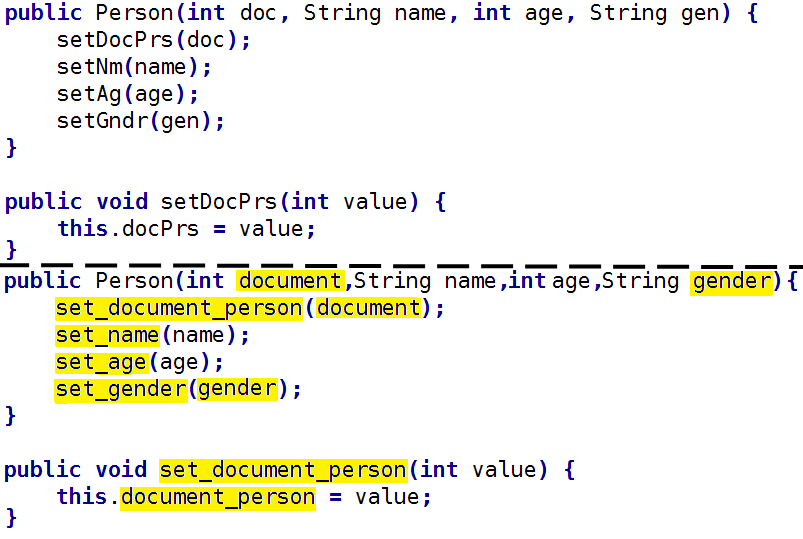
\includegraphics[scale= 0.52]{./cap6/cod.png}
}
\caption{Comparación de un código, antes y después de expandir los Ids}
\label{cod}
\end{figure}

\subsection{Expandir Identificadores en el Código}

Para ubicarse en el contexto de esta mejora, IDA tiene un panel (Panel de Elementos Capturados - Ver Capítulo 4) en donde se visualiza el código del archivo ingresado para que el usuario lo visualice. 

%Este código se resalta los id con color, cuando se seleccionaba un id en la tabla correspondiente (también lo hace con los comentarios y los literales, ver capítulo 4 para más detalles).

Una propuesta de mejora en la herramienta IDA, consiste en traducir los ids que se muestran en esta visualización del código.
Esta traducción implica reemplazar cada id ubicado en el código por la expansión que fue llevada a cabo, dado que hay dos tipos de expansiones por cada id (expansión desde Greedy/Samurai), lo que se permitirá es que el usuario pueda elegir entre ambas alternativas la que mejor le parezca. De esta forma, se obtendrá un código más legible y ayudará a comprenderlo más fácilmente. En la Figura \ref{cod} se explaya esta idea, aquí se compara un código, antes y después de expandir los ids.

Luego el nuevo código con los ids expandidos se podrá guardar en un nuevo archivo de salida JAVA, este nuevo archivo será funcionalmente equivalente al archivo ingresado, pero tendrá los ids expandidos. Esta idea de traducción y creación de un nuevo archivo, fue tomada de una de las características que posee la herramienta Identifier Restructuring cuyos autores son Tonella y Caprile (Ver capitulo 3 - sección \ref{sec:algRest}), ya que esta herramienta realiza una traducción similar de ids generando un código más comprensivo.

\subsection{Acoplar a Entornos de Desarrollo}

Una interesante extensión futura para la herramienta IDA, consiste en adaptarla como extensión (plugin) para un entorno de desarrollo integrado, como es el caso de NetBeans o Eclipse. Esto permitiría que el usuario abra un proyecto JAVA desde estos entornos, e inmediatamente con IDA expanda los ids para mejorar la comprensión. Esta propuesta, en parte es similar a una de la características de la herramienta Identifier Dictionary (IDD), que fue desarrollada por Deissenboeck y Pizka (Ver Capítulo 3 - sección \ref{sec:algIdDic}). La herramienta IDD es un plugin de eclipse que al compilar un proyecto en JAVA, automáticamente captura y enumera dentro de una tabla los ids presentes en el proyecto, luego el usuario puede renombrar cada id desde esta tabla a una forma más comprensiva.

Para la herramienta IDA se propone construir un plugin similar al de IDD, en donde se enumeran los ids en una tabla, pero el renombre de ids en IDA a diferencia de IDD es más automático, ya que IDA expande los ids por medio de las estrategias que tiene implementadas. El usuario solo deberá intervenir para determinar que expansión es la más adecuada, entre los distintos resultados que se obtengan, producto de las diferentes estrategias de análisis de ids ejecutadas.


